
\documentclass[11pt]{article}
\usepackage[margin=1in]{geometry}
\usepackage[T1]{fontenc}
\usepackage{lmodern}
\usepackage{xcolor}
\usepackage{booktabs}
\usepackage{longtable}
\usepackage{array}
\usepackage{enumitem}
\usepackage{hyperref}
\usepackage{listings}
\usepackage{tikz}
\usetikzlibrary{arrows.meta,positioning,calc}

\hypersetup{
  colorlinks=true,
  linkcolor=blue!50!black,
  urlcolor=blue!50!black
}

\lstset{
  basicstyle=\ttfamily\small,
  breaklines=true,
  frame=single,
  columns=fullflexible,
  keepspaces=true,
  showstringspaces=false,
  keywordstyle=\color{blue!60!black},
  commentstyle=\color{green!35!black}
}

\newcommand{\code}[1]{\texttt{\detokenize{#1}}}

\title{FPGA--SN65HVD230--ELM327 CAN/OBD-II Debug Report}
\author{Workspace: \code{/home/andy/verilog_workspace/assume_board_is_nexys3}}
\date{Final successful test: 2026-06-07, Asia/Taipei}

\begin{document}
\maketitle

\section{Executive Summary}

The system is now working.  The FPGA, through an SN65HVD230 CAN transceiver,
responds to an ELM327 adapter on 11-bit, 500 kbit/s OBD-II CAN.  The final
successful ELM327 test returned:

\begin{lstlisting}[language={}]
0100: 7E806410000180000
010C: 7E804410C2EE0
010D: 7E803410D58
\end{lstlisting}

The implemented dummy ECU behavior is:

\begin{center}
\begin{tabular}{lll}
\toprule
Request & Response & Meaning \\
\midrule
\code{0100} & \code{7E8 06 41 00 00 18 00 00} & PID 0C and PID 0D supported \\
\code{010C} & \code{7E8 04 41 0C 2E E0} & RPM = \code{0x2EE0}/4 = 3000 RPM \\
\code{010D} & \code{7E8 03 41 0D 58} & Speed = \code{0x58} = 88 km/h \\
\bottomrule
\end{tabular}
\end{center}

The root cause was hardware wiring: CAN high/low were misplaced relative to
the SN65HVD230/ELM327 bus.  Before the fix, the ELM side could produce
differential activity, but the SN65 RXD input into the FPGA did not see valid
CAN edges.  After correcting the high/low placement, the passive FPGA listener
changed from idle-only output to activity output, and the active OBD responder
successfully answered the ELM327.

\section{Current System Behavior}

\subsection{Protocol and IDs}

The active bitstream currently programs the FPGA as a small OBD-II ECU:

\begin{itemize}[nosep]
  \item CAN bitrate: 500 kbit/s.
  \item CAN frame format: standard 11-bit data frames.
  \item Accepted request IDs: functional \code{0x7DF} and physical \code{0x7E0}.
  \item Response ID: \code{0x7E8}.
  \item Accepted service: mode \code{01} current data.
  \item Supported PIDs: \code{00}, \code{0C}, and \code{0D}.
\end{itemize}

\subsection{Debug UART Behavior}

The CP2102 debug UART is 9600 baud.  Its FPGA output is intentionally inverted
in the top level:

\begin{lstlisting}[language=Verilog]
assign uart_tx_cp2102_inv = ~dbg_uart_tx;
\end{lstlisting}

This inversion is required by the current wiring/debug path.

The active OBD node prints two kinds of debug messages:

\begin{description}[leftmargin=3cm,style=nextline]
  \item[Heartbeat] \code{H<rx><edge><sof><ack><ok><crc_err><stuff><att><tx_ack><done><busy>}
  once per second.
  \item[OBD request] \code{R<pid_byte>} when a supported OBD request is decoded.
  The PID byte is raw binary, so PID \code{00}, \code{0C}, and \code{0D} may not
  print as ordinary visible characters.
\end{description}

Heartbeat fields are:

\begin{center}
\begin{tabular}{ll}
\toprule
Field & Meaning \\
\midrule
\code{rx} & Current SN65 RXD logic level seen by FPGA \\
\code{edge} & Any CAN RX edge since last heartbeat \\
\code{sof} & CAN receiver saw start-of-frame \\
\code{ack} & CAN receiver reached ACK slot while receiving a frame \\
\code{ok} & CRC-valid standard data frame received \\
\code{crc_err} & CRC or format rejection seen \\
\code{stuff} & Bit stuffing error seen \\
\code{att} & FPGA attempted a transmit since last heartbeat \\
\code{tx_ack} & Another CAN node ACKed the FPGA transmit \\
\code{done} & FPGA transmit completed \\
\code{busy} & CAN controller is currently busy \\
\bottomrule
\end{tabular}
\end{center}

During the final successful run, the CP2102 log included:

\begin{lstlisting}[language={}]
H10000000000
R<00>
R<0C>
R<0D>
H11111001110
H10000000100
\end{lstlisting}

The important heartbeat was \code{H11111001110}: RX edges were seen, SOF was
seen, the receiver reached ACK slot, CRC was OK, a transmit was attempted, the
transmit was ACKed by the ELM327, and transmit completed.

\section{Final Wiring}

\subsection{Pin and Signal Map}

The names \code{uart_tx_can} and \code{uart_rx_can} are historical/misleading.
The verified final mapping is:

\begin{longtable}{llll}
\toprule
FPGA pin & Verilog net & Direction at FPGA & External connection \\
\midrule
\endhead
\code{U10} & \code{clk_in} & input & 100 MHz board clock \\
\code{N15} & \code{uart_tx_can} & input & SN65HVD230 \code{RXD} \\
\code{P15} & \code{uart_rx_can} & output & SN65HVD230 \code{TXD} \\
\code{U17} & \code{uart_tx_cp2102_inv} & output & CP2102 RX/debug UART, inverted \\
\code{P16} & \code{uart_rx_cp2102} & input & CP2102 TX, currently unused by OBD node \\
\code{D11} & \code{slow_blink_clk_led} & output & slow heartbeat LED \\
\code{C11} & \code{unused_led} & output & held low \\
\code{T18} & \code{unused_out} & output & held low \\
\bottomrule
\end{longtable}

The B8 direct CANL probe was removed.  It was not a useful final debug method
because CANH/CANL are differential analog bus lines, and connecting one side
directly to a digital FPGA input does not meaningfully decode the CAN bus.

\subsection{TikZ Wiring Diagram}

\begin{center}
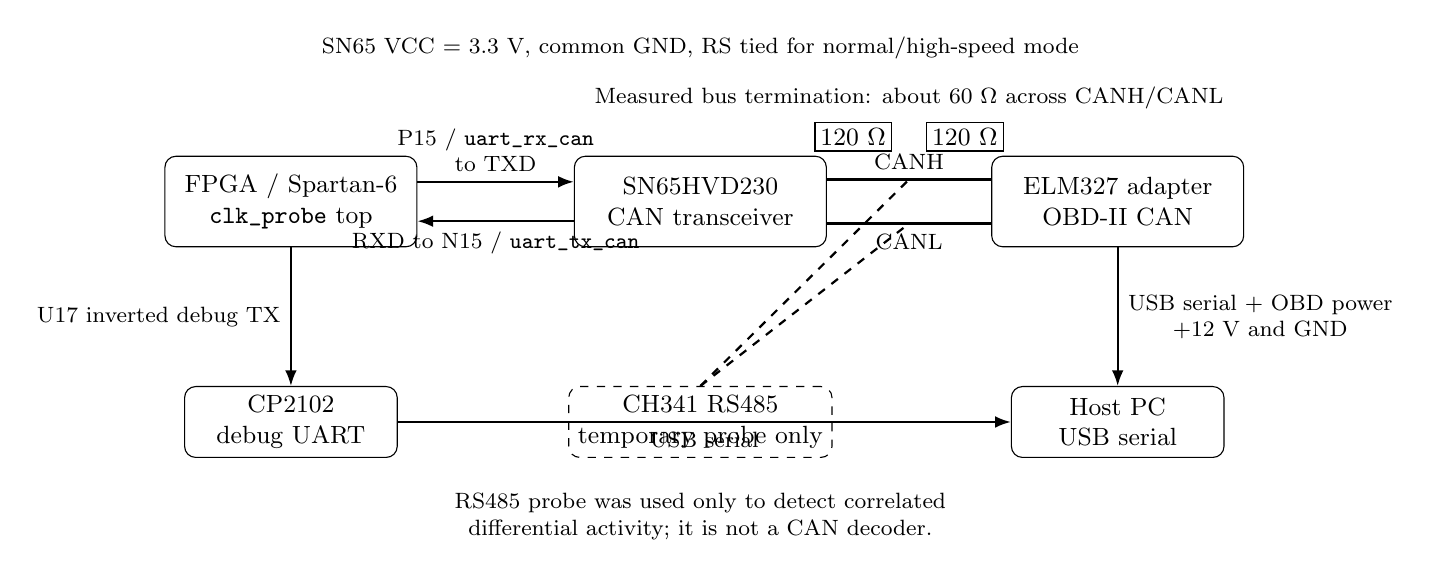
\begin{tikzpicture}[
  font=\small,
  block/.style={draw, rounded corners, align=center, minimum width=3.2cm, minimum height=1.15cm},
  smallblock/.style={draw, rounded corners, align=center, minimum width=2.7cm, minimum height=0.9cm},
  wire/.style={-{Latex[length=2mm]}, thick},
  bus/.style={thick},
  probe/.style={dashed, thick},
  note/.style={align=center, font=\footnotesize}
]

\node[block] (fpga) at (0,0) {FPGA / Spartan-6\\\code{clk_probe} top};
\node[block] (sn65) at (5.2,0) {SN65HVD230\\CAN transceiver};
\node[block] (elm) at (10.5,0) {ELM327 adapter\\OBD-II CAN};
\node[smallblock] (cp) at (0,-2.8) {CP2102\\debug UART};
\node[smallblock] (host) at (10.5,-2.8) {Host PC\\USB serial};
\node[smallblock, dashed] (ch341) at (5.2,-2.8) {CH341 RS485\\temporary probe only};

\draw[wire] ([yshift=0.25cm]fpga.east) -- node[above,note]{P15 / \code{uart_rx_can}\\to TXD} ([yshift=0.25cm]sn65.west);
\draw[wire] ([yshift=-0.25cm]sn65.west) -- node[below,note]{RXD to N15 / \code{uart_tx_can}} ([yshift=-0.25cm]fpga.east);

\draw[bus] ([yshift=0.28cm]sn65.east) -- node[above,note]{CANH} ([yshift=0.28cm]elm.west);
\draw[bus] ([yshift=-0.28cm]sn65.east) -- node[below,note]{CANL} ([yshift=-0.28cm]elm.west);

\node[draw, fill=white, inner sep=2pt] at ($(sn65.east)!0.16!(elm.west)+(0,0.82)$) {$120~\Omega$};
\node[draw, fill=white, inner sep=2pt] at ($(sn65.east)!0.84!(elm.west)+(0,0.82)$) {$120~\Omega$};
\node[note] at ($(sn65.east)!0.50!(elm.west)+(0,1.32)$) {Measured bus termination: about $60~\Omega$ across CANH/CANL};

\draw[wire] (fpga.south) -- node[left,note]{U17 inverted debug TX} (cp.north);
\draw[wire] (cp.east) -- node[below,note]{USB serial} (host.west);
\draw[wire] (elm.south) -- node[right,note]{USB serial + OBD power\\+12 V and GND} (host.north);

\draw[probe] (ch341.north) -- ($(sn65.east)!0.50!(elm.west)+(0,0.28)$);
\draw[probe] (ch341.north) -- ($(sn65.east)!0.50!(elm.west)+(0,-0.28)$);
\node[note] at (5.2,-4.0) {RS485 probe was used only to detect correlated\\differential activity; it is not a CAN decoder.};

\node[note] at (5.2,1.95) {SN65 VCC = 3.3 V, common GND, RS tied for normal/high-speed mode};

\end{tikzpicture}
\end{center}

\section{Source File Manual}

\begin{longtable}{p{0.26\textwidth}p{0.68\textwidth}}
\toprule
File & Purpose \\
\midrule
\endhead
\code{index.v} & Top-level FPGA module \code{clk_probe}.  Instantiates \code{obd_can_node}, maps SN65 RXD/TXD, preserves the required CP2102 debug inversion, drives LEDs/unused outputs.  Edit this file when changing top-level wiring or replacing the active OBD node with a temporary debug module. \\
\code{blink.ucf} & Xilinx UCF pin constraints.  Current CAN pins are N15 = SN65 RXD input and P15 = SN65 TXD output.  B8 is intentionally absent.  Edit this file only when physical pin assignments change. \\
\code{obd_can_node.v} & OBD-II application layer.  Filters request IDs \code{0x7DF}/\code{0x7E0}, recognizes service \code{01}, supports PIDs \code{00}, \code{0C}, and \code{0D}, and formats responses from ID \code{0x7E8}.  Also generates CP2102 debug output. \\
\code{can_simple_controller.v} & Simple standard-frame CAN controller.  Handles bit timing, receive parsing, CRC, bit stuffing, ACK slot drive, transmit frame preparation, and transmit ACK detection.  Edit this carefully; most physical/debug issues should be isolated before changing this file. \\
\code{uart_tx.v} & UART transmitter used by debug output.  Current debug baud is 9600.  The top-level inverts its output for the CP2102 path. \\
\code{doall.sh} & Build/program script.  Sources Xilinx ISE 14.7 settings, opens \code{assume_board_is_nexys3.xise}, runs synthesize/implement/bitgen, writes \code{burn.cmd}, and programs \code{clk_probe.bit} with iMPACT. \\
\code{cp2102workspace/cp2102_recv_uart.py} & Reads a serial port and prints debug UART characters.  Use for CP2102 debug output. \\
\code{cp2102workspace/cp2102_send_bits.py} & Old helper that repeatedly sends one packed byte over serial.  It is not needed for the current OBD responder flow. \\
\code{assume_board_is_nexys3.xise} & Xilinx ISE project file used by \code{doall.sh}. \\
\code{clk_probe.bit} & Generated bitstream that is programmed to the FPGA. \\
\bottomrule
\end{longtable}

\section{Build and Run Manual}

\subsection{Find the Serial Ports}

USB serial numbering can change.  Check stable symlinks first:

\begin{lstlisting}[language=bash]
ls -l /dev/serial/by-id /dev/serial/by-path
ls -l /dev/ttyUSB* /dev/ttyACM*
\end{lstlisting}

During the successful run, the mapping was:

\begin{center}
\begin{tabular}{lll}
\toprule
Device & Observed port & Serial settings \\
\midrule
ELM327 / FTDI & \code{/dev/ttyUSB0} & 38400 baud \\
CP2102 debug UART & \code{/dev/ttyUSB2} & 9600 baud \\
Digilent/JTAG serial & \code{/dev/ttyUSB3} & not used for OBD test \\
CH341 RS485 probe & \code{/dev/ttyUSB1} when connected & 500000 baud for activity probe only \\
\bottomrule
\end{tabular}
\end{center}

If permission is needed, run commands through the \code{dialout} group, as was
done during debug:

\begin{lstlisting}[language=bash]
sg dialout -c "<command>"
\end{lstlisting}

\subsection{Compile and Program the FPGA}

The normal build/program command is:

\begin{lstlisting}[language=bash]
cd /home/andy/verilog_workspace/assume_board_is_nexys3
sg dialout -c "./doall.sh"
\end{lstlisting}

\code{doall.sh} performs these operations:

\begin{enumerate}[nosep]
  \item Source \code{/opt/Xilinx/14.7/ISE_DS/settings64.sh}.
  \item Open \code{assume_board_is_nexys3.xise} with \code{xtclsh}.
  \item Run \code{Synthesize - XST}.
  \item Run \code{Implement Design}.
  \item Run \code{Generate Programming File} to create \code{clk_probe.bit}.
  \item Create \code{burn.cmd}.
  \item Program the FPGA through Digilent/iMPACT.
\end{enumerate}

A successful program operation ends with text similar to:

\begin{lstlisting}[language={}]
INFO:iMPACT:188 - '1': Programming completed successfully.
'1': Programmed successfully.
\end{lstlisting}

\subsection{Monitor FPGA Debug Output}

Start CP2102 debug capture:

\begin{lstlisting}[language=bash]
sg dialout -c "python3 cp2102workspace/cp2102_recv_uart.py --port /dev/ttyUSB2 --baud 9600"
\end{lstlisting}

Idle active-firmware output should look like:

\begin{lstlisting}[language={}]
H10000000000
H10000000000
\end{lstlisting}

\subsection{Run the ELM327 OBD Test}

The manual ELM command sequence is:

\begin{lstlisting}[language={}]
ATZ
ATE0
ATL0
ATS0
ATH1
ATSP6
ATCAF1
ATRV
0100
010C
010D
ATBD
\end{lstlisting}

A Python version used during the successful test was:

\begin{lstlisting}[language=Python]
import serial, time
ser = serial.Serial('/dev/ttyUSB0', 38400, timeout=0.25)
time.sleep(0.1)
ser.reset_input_buffer()

def send(cmd, wait=2.0):
    ser.reset_input_buffer()
    ser.write((cmd + '\r').encode())
    end = time.time() + wait
    data = bytearray()
    while time.time() < end:
        b = ser.read(1)
        if b:
            data.extend(b)
            if b == b'>':
                break
    print(cmd + ': ' + data.decode(errors='replace').replace('\r', '\\r').replace('\n', '\\n'))

for c in ['ATZ', 'ATE0', 'ATL0', 'ATS0', 'ATH1', 'ATSP6', 'ATCAF1',
          'ATRV', '0100', '010C', '010D', 'ATCS', 'ATBD']:
    send(c, 2.5)
ser.close()
\end{lstlisting}

Expected successful response:

\begin{lstlisting}[language={}]
ATRV: 11.8V
0100: 7E806410000180000
010C: 7E804410C2EE0
010D: 7E803410D58
ATBD: 0C 00 00 07 E8 03 41 0D 58 00 00 00 00
\end{lstlisting}

\section{What Was Wrong}

The failure was not primarily the Verilog OBD response data.  The key problem
was physical CAN wiring: CANH/CANL placement was wrong at some point in the
chain, so the SN65HVD230 side did not see the ELM327 bus correctly.

The strongest evidence was the combination of these observations:

\begin{itemize}[nosep]
  \item Before the final fix, ELM commands such as \code{0100}, \code{010C}, and
  \code{010D} returned \code{CAN ERROR}.
  \item A passive FPGA/SN65 listener repeatedly printed \code{R10000}, meaning
  SN65 RXD stayed high and no edges/lows were observed.
  \item The CH341 RS485 differential probe saw bursts correlated with ELM
  requests, proving some differential activity existed on the ELM/probe pair.
  \item At the same time, the FPGA/SN65 RXD did not see that activity, proving
  the SN65/FPGA path was not on the same valid CAN signal polarity/pair.
  \item A temporary FPGA pulse through SN65 TXD was seen locally on SN65 RXD but
  not by the CH341 probe, again pointing to a bus-side wiring mismatch rather
  than only a Verilog parser issue.
\end{itemize}

After correcting the high/low placement, the passive listener changed to
\code{R111FF} during an ELM request window.  That meant RXD saw edges and
dominant lows.  Then the active responder immediately produced valid ELM
responses.

\section{Debug Timeline and Attempts}

\begin{enumerate}
  \item Read the existing project notes in \code{doing_stuff.txt} and verified
  that \code{blink.ucf} was the authoritative pin source.
  \item Reconfirmed the final FPGA/SN65 pin interpretation: N15 is CAN RX into
  FPGA from SN65 RXD, and P15 is CAN TX from FPGA to SN65 TXD.
  \item Reconnected a loose CAN TX pin.  This did not yet make ELM requests work.
  \item Provided ELM327 OBD-side 12 V and ground.  \code{ATRV} then showed about
  \code{11.8V}, but requests still returned \code{CAN ERROR}.
  \item Added the second 120 \(\Omega\) CAN terminator.  The bus then measured
  about 60 \(\Omega\) across CANH/CANL, which is the expected value for two
  120 \(\Omega\) terminators in parallel.
  \item Tried CANH/CANL swaps and wire adjustments.  Earlier attempts still did
  not produce valid SN65 RXD activity.
  \item Programmed a passive raw listener that held FPGA CAN TX recessive
  forever.  This answered the question of whether the FPGA/FFmpeg-like logic
  could listen without sending: yes, the FPGA can listen passively through the
  SN65 RXD pin, but before the hardware fix it saw no ELM activity.
  \item Added a direct B8-to-CANL debug probe and a UCF pin for it.  This was
  later removed because a single-ended digital FPGA input is not a meaningful
  CAN differential receiver.
  \item Added a CH341 RS485 adapter as a temporary differential activity probe.
  It was useful only as a rough edge/activity detector, not as a CAN decoder.
  At 500000 baud it saw byte bursts correlated with ELM request timing.
  \item Programmed a one-millisecond-per-second SN65 dominant pulse diagnostic.
  This proved the local FPGA/SN65 TXD/RXD side could react, but the pulse was
  not seen by the CH341 probe, strengthening the bus-side wiring diagnosis.
  \item Corrected the CANH/CANL placement in hardware.
  \item Reprogrammed the passive listener with B8 removed and CAN TX held
  recessive.  It changed from \code{R10000} idle/no activity to \code{R111FF}
  during ELM request activity.
  \item Reprogrammed the active OBD responder, disabled the old periodic test TX,
  and verified successful ELM responses for \code{0100}, \code{010C}, and
  \code{010D}.
\end{enumerate}

\section{Current Code Configuration}

The final source state is intentionally simple:

\begin{itemize}[nosep]
  \item \code{index.v} instantiates \code{obd_can_node} directly.
  \item \code{blink.ucf} has 8 constrained I/O pins and no B8 probe.
  \item \code{obd_can_node.v} has \code{TEST_TX_ENABLE = 1'b0}, so it does not
  send periodic diagnostic frames.
  \item The FPGA only transmits when a supported OBD request is decoded, or when
  the CAN controller drives the ACK slot for a valid received frame.
\end{itemize}

\section{Practical Notes for Future Work}

\begin{itemize}
  \item If ELM requests return \code{CAN ERROR} again, first run the passive
  listener style test or inspect the active heartbeat.  If there are no RX
  edges, debug hardware before changing the CAN parser.
  \item Keep the CP2102 debug inversion in \code{index.v}.  Removing it causes
  unreadable debug output with the current wiring.
  \item Use \code{/dev/serial/by-id} to identify USB serial adapters.  The
  \code{/dev/ttyUSBx} numbers changed during debug.
  \item Do not use the CH341 RS485 adapter as a CAN decoder.  It can show
  correlated activity, but CAN framing, arbitration, stuffing, CRC, and ACK are
  not RS485 UART protocol.
  \item Keep CAN termination at two 120 \(\Omega\) endpoints.  A powered-down or
  disconnected setup should still measure about 60 \(\Omega\) across CANH/CANL
  when both terminators are present.
  \item If adding more PIDs, edit the supported PID mask and response case in
  \code{obd_can_node.v}.  The current dummy data is deliberately fixed.
\end{itemize}

\end{document}
